\documentclass[12pt,a4paper,openany]{book}
\usepackage{lmodern}
\usepackage[svgnames]{xcolor} % Required to specify font color
\input{/home/aroquemaurel/cours/includesLaTeX/couleurs.tex}

\usepackage[utf8]{inputenc} \usepackage[T1]{fontenc}
\usepackage[francais]{babel}
\usepackage[top=1.7cm, bottom=1.7cm, left=1.7cm, right=1.7cm]{geometry}
\usepackage{verbatim}
\usepackage[urlbordercolor={1 1 1}, linkbordercolor={1 1 1}, linkcolor=vert1, urlcolor=bleu, colorlinks=true]{hyperref}
\usepackage{tikz} %Vectoriel
\usepackage{listings}
\usepackage{fancyhdr}
\usepackage{multido}
\usepackage{float}
\usepackage{amssymb}
\usepackage{longtable}
\usepackage{wrapfig}

\newcommand{\titre}{Projet de programmation}
\newcommand{\subtitle}{Partie Java}
\newcommand{\auteur}{Antoine de \bsc{Roquemaurel} et Dario \bsc{Olibet}}
\newcommand{\formation}{L3 Informatique}
\newcommand{\semestre}{5}
\newcommand{\annee}{2013}
\newcommand{\prof}{}


\newcommand{\pole}{}
\newcommand{\sigle}{pf1}


\input{/home/aroquemaurel/cours/includesLaTeX/listings.tex}
\date{\today}

\makeindex
\lfoot{Université Toulouse III -- Paul Sabatier}
\rfoot{}
%\rfoot{}
\cfoot{}
\makeglossary
\makeatletter
\def\clap#1{\hbox to 0pt{\hss #1\hss}}%
\def\ligne#1{%
\hbox to \hsize{%
\vbox{\centering #1}}}%
\def\haut#1#2#3{%
\hbox to \hsize{%
\rlap{\vtop{\raggedright #1}}%
\hss
\clap{\vtop{\centering #2}}%
\hss
\llap{\vtop{\raggedleft #3}}}}%
\def\bas#1#2#3{%
\hbox to \hsize{%
\rlap{\vbox{\raggedright #1}}%
\hss \clap{\vbox{\centering #2}}%
\hss
\llap{\vbox{\raggedleft #3}}}}%
\def\maketitle{%
\thispagestyle{empty}\vbox to \vsize{%
\haut{}{\@blurb}{}

\vfill
\vspace{1cm}
\begin{flushleft}
\usefont{OT1}{ptm}{m}{n}
\huge \@title
\end{flushleft}
\par
\hrule height 4pt
\par
\begin{flushright}
\usefont{OT1}{phv}{m}{n}
\Large \@author
\par
\end{flushright}
\vspace{1cm}
\vfill
\vfill
\bas{}{\@location, le \@date}{}
}%
\cleardoublepage
}
\def\date#1{\def\@date{#1}}
\def\author#1{\def\@author{#1}}
\def\title#1{\def\@title{#1}}
\def\location#1{\def\@location{#1}}
\def\blurb#1{\def\@blurb{#1}}
\date{\today}
\author{}
\title{}
\location{Amiens}\blurb{}
\makeatother
\title{\titre}
\author{Partie Java}

\location{Toulouse}
\blurb{%
Université Toulouse III -- Paul sabatier\\
L3 Informatique\\
\vspace{30px}
\begin{flushleft}Antoine de \bsc{Roquemaurel} \\ 
	Dario \bsc{Olibet} \\
 Groupe 1.1\end{flushleft}
}%



%\title{Cours \\ \titre}
%\date{\today\\ Semestre \semestre}

%\lhead{Cours: \titre}
%\chead{}
%\rhead{\thepage}

%\lfoot{Université Paul Sabatier Toulouse III}
%\cfoot{\thepage}
%\rfoot{\sigle\semestre}

\pagestyle{fancy}
\renewcommand{\chaptermark}[1]{\markboth{\bsc{\chaptername~\thechapter{} :} #1}{}}
\renewcommand{\sectionmark}[1]{\markright{\thesection{ #1}}}
\renewcommand{\headrulewidth}{0.3pt}
\renewcommand{\footrulewidth}{0.3pt}

\fancyhf{}
\fancyhead[LE]{\leftmark}
\fancyhead[RO]{\rightmark}
\fancyfoot[LE,RO]{--~\thepage~--}
\fancyfoot[LO]{\titre{}}
\fancyfoot[RE]{Antoine de \bsc{Roquemaurel} -- Dario \bsc{Olibet}}

%% Cas des premières pages de chapitre
\fancypagestyle{plain}{%
	\fancyhf{}%
	\fancyfoot[L]{\titre{}}
	\fancyfoot[R]{--~\thepage~--}
	\renewcommand{\headrulewidth}{0pt}
	\renewcommand{\footrulewidth}{0.3pt}
}
\makeatletter
\renewcommand*{\lstlistlistingname}{Liste des codes sources}
\renewcommand\listoffigures{%
    \chapter{\listfigurename}%
      \@mkboth{\MakeUppercase\listfigurename}%
              {\MakeUppercase\listfigurename}%
       \@starttoc{lof}%
    }
    \renewcommand\listoftables{%
    \chapter{\listtablename}%
    \@mkboth{\MakeUppercase{\listtablename}}%
            {\MakeUppercase{\listtablename}}%
    \@starttoc{lot}
    }

    \renewcommand\lstlistoflistings{%
    \begingroup
    \chapter{\lstlistlistingname}%
    \parskip\z@\parindent\z@\parfillskip \z@ \@plus 1fil%
    \@starttoc{lol}%
    \endgroup
    }
	\makeatother

\input{/home/aroquemaurel/cours/includesLaTeX/remarquesExempleAttention.tex}
\input{/home/aroquemaurel/cours/includesLaTeX/polices.tex}
\input{/home/aroquemaurel/cours/includesLaTeX/affichageChapitre.tex}
%\let\pagebreakORIG\pagebreak
%\let\clearpageORIG\clearpage
%\let\cleardoublepageORIG\cleardoublepage

%\ifx \removepagebreak \undefined
%\newcommand{\removepagebreak}{\renewcommand{\pagebreak}{}\renewcommand{\clearpage}{}\renewcommand{\cleardoublepage}{}}
%\fi
%
%\ifx \restorepagebreak \undefined
%%\newcommand{\restorepagebreak}{\renewcommand{\pagebreak}{\pagebreakORIG}\renewcommand{\clearpage}{\clearpageORIG}\renewcommand{\cleardoublepage}{\cleardoublepageORIG}}
%
%\fi
%\newcommand{\pfp}{\texttt{pfp}}

%\newcommand{\ifp}{\texttt{if}}
%\newcommand{\elsep}{\texttt{else}}

\makeatother
\includeonly {
}
\newcommand{\bootstrap}{\textit{bootstrap}}
\begin{document}
	\setcounter{tocdepth}{2}
	\setcounter{secnumdepth}{3}
	\maketitle
	\newpage
	\chapter*{Avant-propos}
	Ce dossier comporte l'organisation et les étapes de développement d'un projet d'Arènes en Java. 

	Il à été conçut par Antoine de \bsc{Roquemaurel} et Dario \bsc{Olibet} dans le cadre du module \textit{Projet de programmation} de la L3
	Informatique de l'université Toulouse III -- Paul Sabatier.\\~

	\large{\sectionfont Contenu de l'archive du projet}\\
	\normalsize
	L'archive que vous avez reçus était organisée comme ceci: 
	\begin{description}
		\item[\texttt{rapport.pdf}] Le présent rapport que vous êtes en train de lire
		\item[\texttt{V1/}] Contient le dossier avec la première version de l'application : notre propre arènes avec les règles que nous avons implémentées. 
		\item[\texttt{V1/doc/}] Contient la documentation de la première version du projet. Celle-ci à été générée à l'aide de \textit{Doxygen}, elle
			est disponible en HTML ou en PDF (générée avec \LaTeX).

			L'utilisation de \textit{Doxygen} contrairement à \textit{Javadoc} permet d'avoir une génération en PDF, mais également d'avoir l'apparition des diagrammes de
			classes.
		\item[\texttt{V2/}] Contient le dossier avec la version contenant notre strategie pour l'arène commune distante.
	\end{description}

	Le projet à été développé en Java6.

	\vfill
	\footnotesize Rédigé le \today{} par Antoine de \bsc{Roquemaurel} et Dario \bsc{Olibet}
	\tableofcontents
	\chapter{Organisation du travail d'équipe}
	Pour ce projet, nous étions deux à travailler dessus, ainsi nous avons utilisé plusieurs techniques afin de se coordonner et de limiter les problèmes. Ceci
	n'est pas notre premier projet ensemble, notre travail en fut simplifié.
	\section{Un outil de gestion de projet : Redmine}
	\begin{figure}[H]
		\centering
		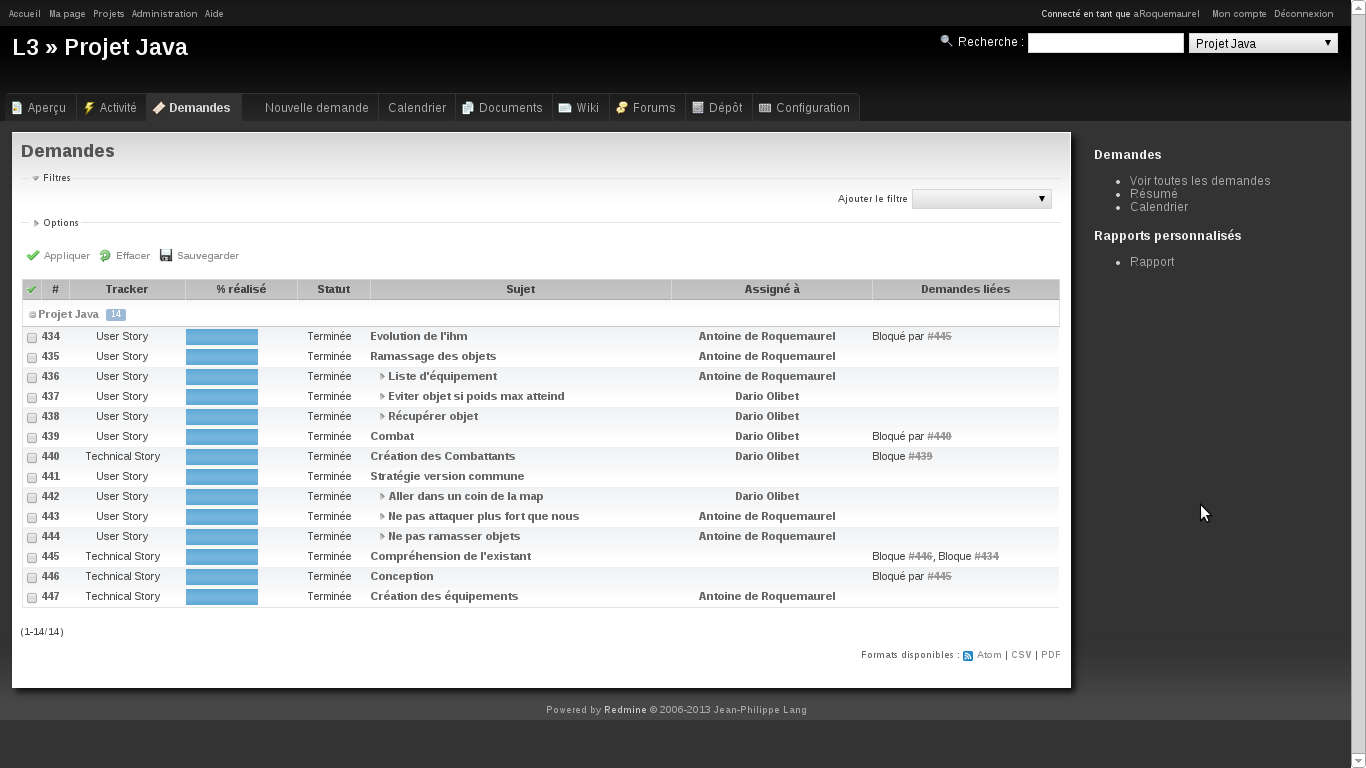
\includegraphics[width=18cm]{screens/redmine.png}
		\caption{Affichage des demandes dans Redmine}
		\label{fig:redmine}
	\end{figure}
	Pour le projet, nous avons utiliser \textit{Redmine}, une plateforme web de gestion de projet (Cf figure \ref{fig:redmine}). Elle nous a permis de simplifier le travail, et
	de ne rien oublier.

	En effet, nous pouvons créer des tâches, signaler qu'elles sont en cours/terminés/en tests, leur donner des dates limites, les affecter à une personne etc\ldots
	Ainsi lorsque l'un de nous commençait une tâche, il le signalait sur le \textit{redmine}, ce qui permettait de tenir au courant son binôme de ses actions et
	de l'avancée du projet.

	\section{Un logiciel de versionnement : Git}
	Afin de limiter les problèmes du travail collaboratif, nous avons utilisé un logiciel de versionnement Git. Il a deux intérêt, tout d'abord, nous pouvons
	travailler à deux en parallèle sur le projet sans se soucier de fusionner notre travail\footnote{À condition de ne pas travailler sur deux lignes de code
	identiques}.

	D'autre part, tous les logs étant enregistrés, nous pouvons savoir qui à fait quoi et quel jour, cela permet de voir également l'avancée du projet. 

	Enfin, toutes les modification sont stockées sur le serveur, ainsi en cas de problème, il est très facile de revenir à la version précédente ou même de
	comparer deux versions afin de voir les changements et de comprendre rapidement pourquoi une fonctionnalité à régressé. 

	\section{Répartition des tâches}
	%% TODO

	\chapter{Première version}
	\section{Nos règles de jeu}
	\section{Conception}

	\chapter{Seconde Version}
	\section{Stratégie}


%	\appendix
%	\listoffigures
%	\removepagebreak
%	\vfill
%	\lstlistoflistings
%	\vfill
%	\restorepagebreak
\end{document}

